\documentclass{article}


% if you need to pass options to natbib, use, e.g.:
%     \PassOptionsToPackage{numbers, compress}{natbib}
% before loading neurips_2022


% ready for submission
% \usepackage{neurips_2022}


% to compile a preprint version, e.g., for submission to arXiv, add add the
% [preprint] option:
\usepackage[preprint]{neurips_2022}


% to compile a camera-ready version, add the [final] option, e.g.:
%     \usepackage[final]{neurips_2022}


% to avoid loading the natbib package, add option nonatbib:
%    \usepackage[nonatbib]{neurips_2022}


\usepackage[utf8]{inputenc} % allow utf-8 input
\usepackage[T1]{fontenc}    % use 8-bit T1 fonts
\usepackage{hyperref}       % hyperlinks
\usepackage{url}            % simple URL typesetting
\usepackage{booktabs}       % professional-quality tables
\usepackage{amsfonts}       % blackboard math symbols
\usepackage{nicefrac}       % compact symbols for 1/2, etc.
\usepackage{microtype}      % microtypography
\usepackage{xcolor}         % colors

\usepackage{bm}
\usepackage{natbib}
\usepackage{graphicx}
\usepackage{float}

\title{TS2VecAR - Adding autoregressive temporal contrasting to an universal representation of a time series}


% The \author macro works with any number of authors. There are two commands
% used to separate the names and addresses of multiple authors: \And and \AND.
%
% Using \And between authors leaves it to LaTeX to determine where to break the
% lines. Using \AND forces a line break at that point. So, if LaTeX puts 3 of 4
% authors names on the first line, and the last on the second line, try using
% \AND instead of \And before the third author name.


\author{%
  Constantin von Crailsheim \\
Department of Statistics\\
  Ludwig-Maximilians-Universtität München
  \texttt{c.crailsheim@campus.lmu.de} \\
  % examples of more authors
  % \And
  % Coauthor \\
  % Affiliation \\
  % Address \\
  % \texttt{email} \\
  % \AND
  % Coauthor \\
  % Affiliation \\
  % Address \\
  % \texttt{email} \\
  % \And
  % Coauthor \\
  % Affiliation \\
  % Address \\
  % \texttt{email} \\
  % \And
  % Coauthor \\
  % Affiliation \\
  % Address \\
  % \texttt{email} \\
}


\begin{document}


\maketitle


\begin{abstract}
While classification of time series data is crucial in various domains, there are only few labelled datasets available. Thus, self-supervised learning provides significant added value to learn the inherent structure of a time series before fine-tuning a classifier. This investigation builds on TS2Vec \citep{ts2vec}, which learns a robust contextual representations of a time series that can be used for several downstream tasks. Inspired by \citet{tstcc}, we add a cross-prediction task of future time stamps using information about previous time stamps as summarised by an autoregressive model. This allows the extended TS2VecAR model to learn more about the structure of the time series. The model outperforms the model on several benchmark datasets, with better average performance on Human Activity Recognition (HAR) datasets. The source code is available at \url{https://github.com/constantin-crailsheim/TS2VecAR}.
\end{abstract}


\section{Introduction and related work}

Time series data play an integral role in science and industry in various fields such as medicine, finance and manufacturing. However, \citet{tstcc} pointed out that human annotation is very challenging since time series patterns are not easily recognisable by humans, hence only few time series data have been labelled \citep{ching2020}. This demonstrates the need for self-supervised learning methods which can learn the structure of an unlabelled time series in a pretext task and thus require only few labelled instances to fine-tune a classifier. \\

Self-supervised representation learning has been particularly popular in computer vision using a contrastive loss function. In contrastive methods, invariant representations of the initial data are learned by inducing similar latent representations for the same instances in a different augmented context and dissimilar latent representations for different instances. \citet{bachman2019} maximize the mutual information between features in multiple views to induce the algorithm to learn higher-level properties of the data. \citet{simclr} propose a simplified contrastive learning framework and highlight the role of data augmentation configurations. \\

Representation learning for time series has recently gained momentum. \citet{franceschi2019} obtained a generic representation by sampling positives as random subseries and feeding these through a dilated convolutional encoder, whereby the latent representations are evaluated with triplet loss. \citet{mohsenvand2020} extended the SimCLR framework \citep{simclr}  to perform a classification task on EEG time series data. \citet{tonekaboni2021} propose a contrastive learning framework for non-stationary time series, where the distribution of local signals should be distinguishable. \citet{oord2018} use an autoregressive model to predict future instances in the latent space to induce representation that captures relevant information for predicting future instances. \\

While previous work has yielded latent representations that satisfy subseries consistency \citep{franceschi2019} and temporal consistency \citep{tonekaboni2021}, \citet{ts2vec} argue that these strong assumptions may be violated in the presence of level shifts and anomalies. Thus, they propose contextual consistency, which simply "treats the representations at the same timestamp in two augmented contexts as a positive pair" \citep[p. 8982]{ts2vec}. Since they showed very strong results in several tasks, we used TS2Vec as the underlying framework for my model implementation. However, TS2Vec only evaluates the quality of the representation of each timestamp in a rather isolated way and does not learn the structure of the time series in an autoregressive sense. Therefore, we integrated the cross-prediction task proposed by \citet{tstcc} in their TS-TCC model into the TS2Vec framework, which uses a context vector summarising a sample of consecutive latent representations with a Transformer \citep{vaswani2017} as autoregressive model to predict future latent representations. With this extension, which we will refer to as TS2VecAR, we aim to derive robust contextual representations that also capture relevant information about future timestamps.

\section{Method}

As shown below, TS2VecAR embeds the temporal contrasting module of TS-TCC into the initial implementation of TS2Vec.

\begin{figure}[H]
  \centering
  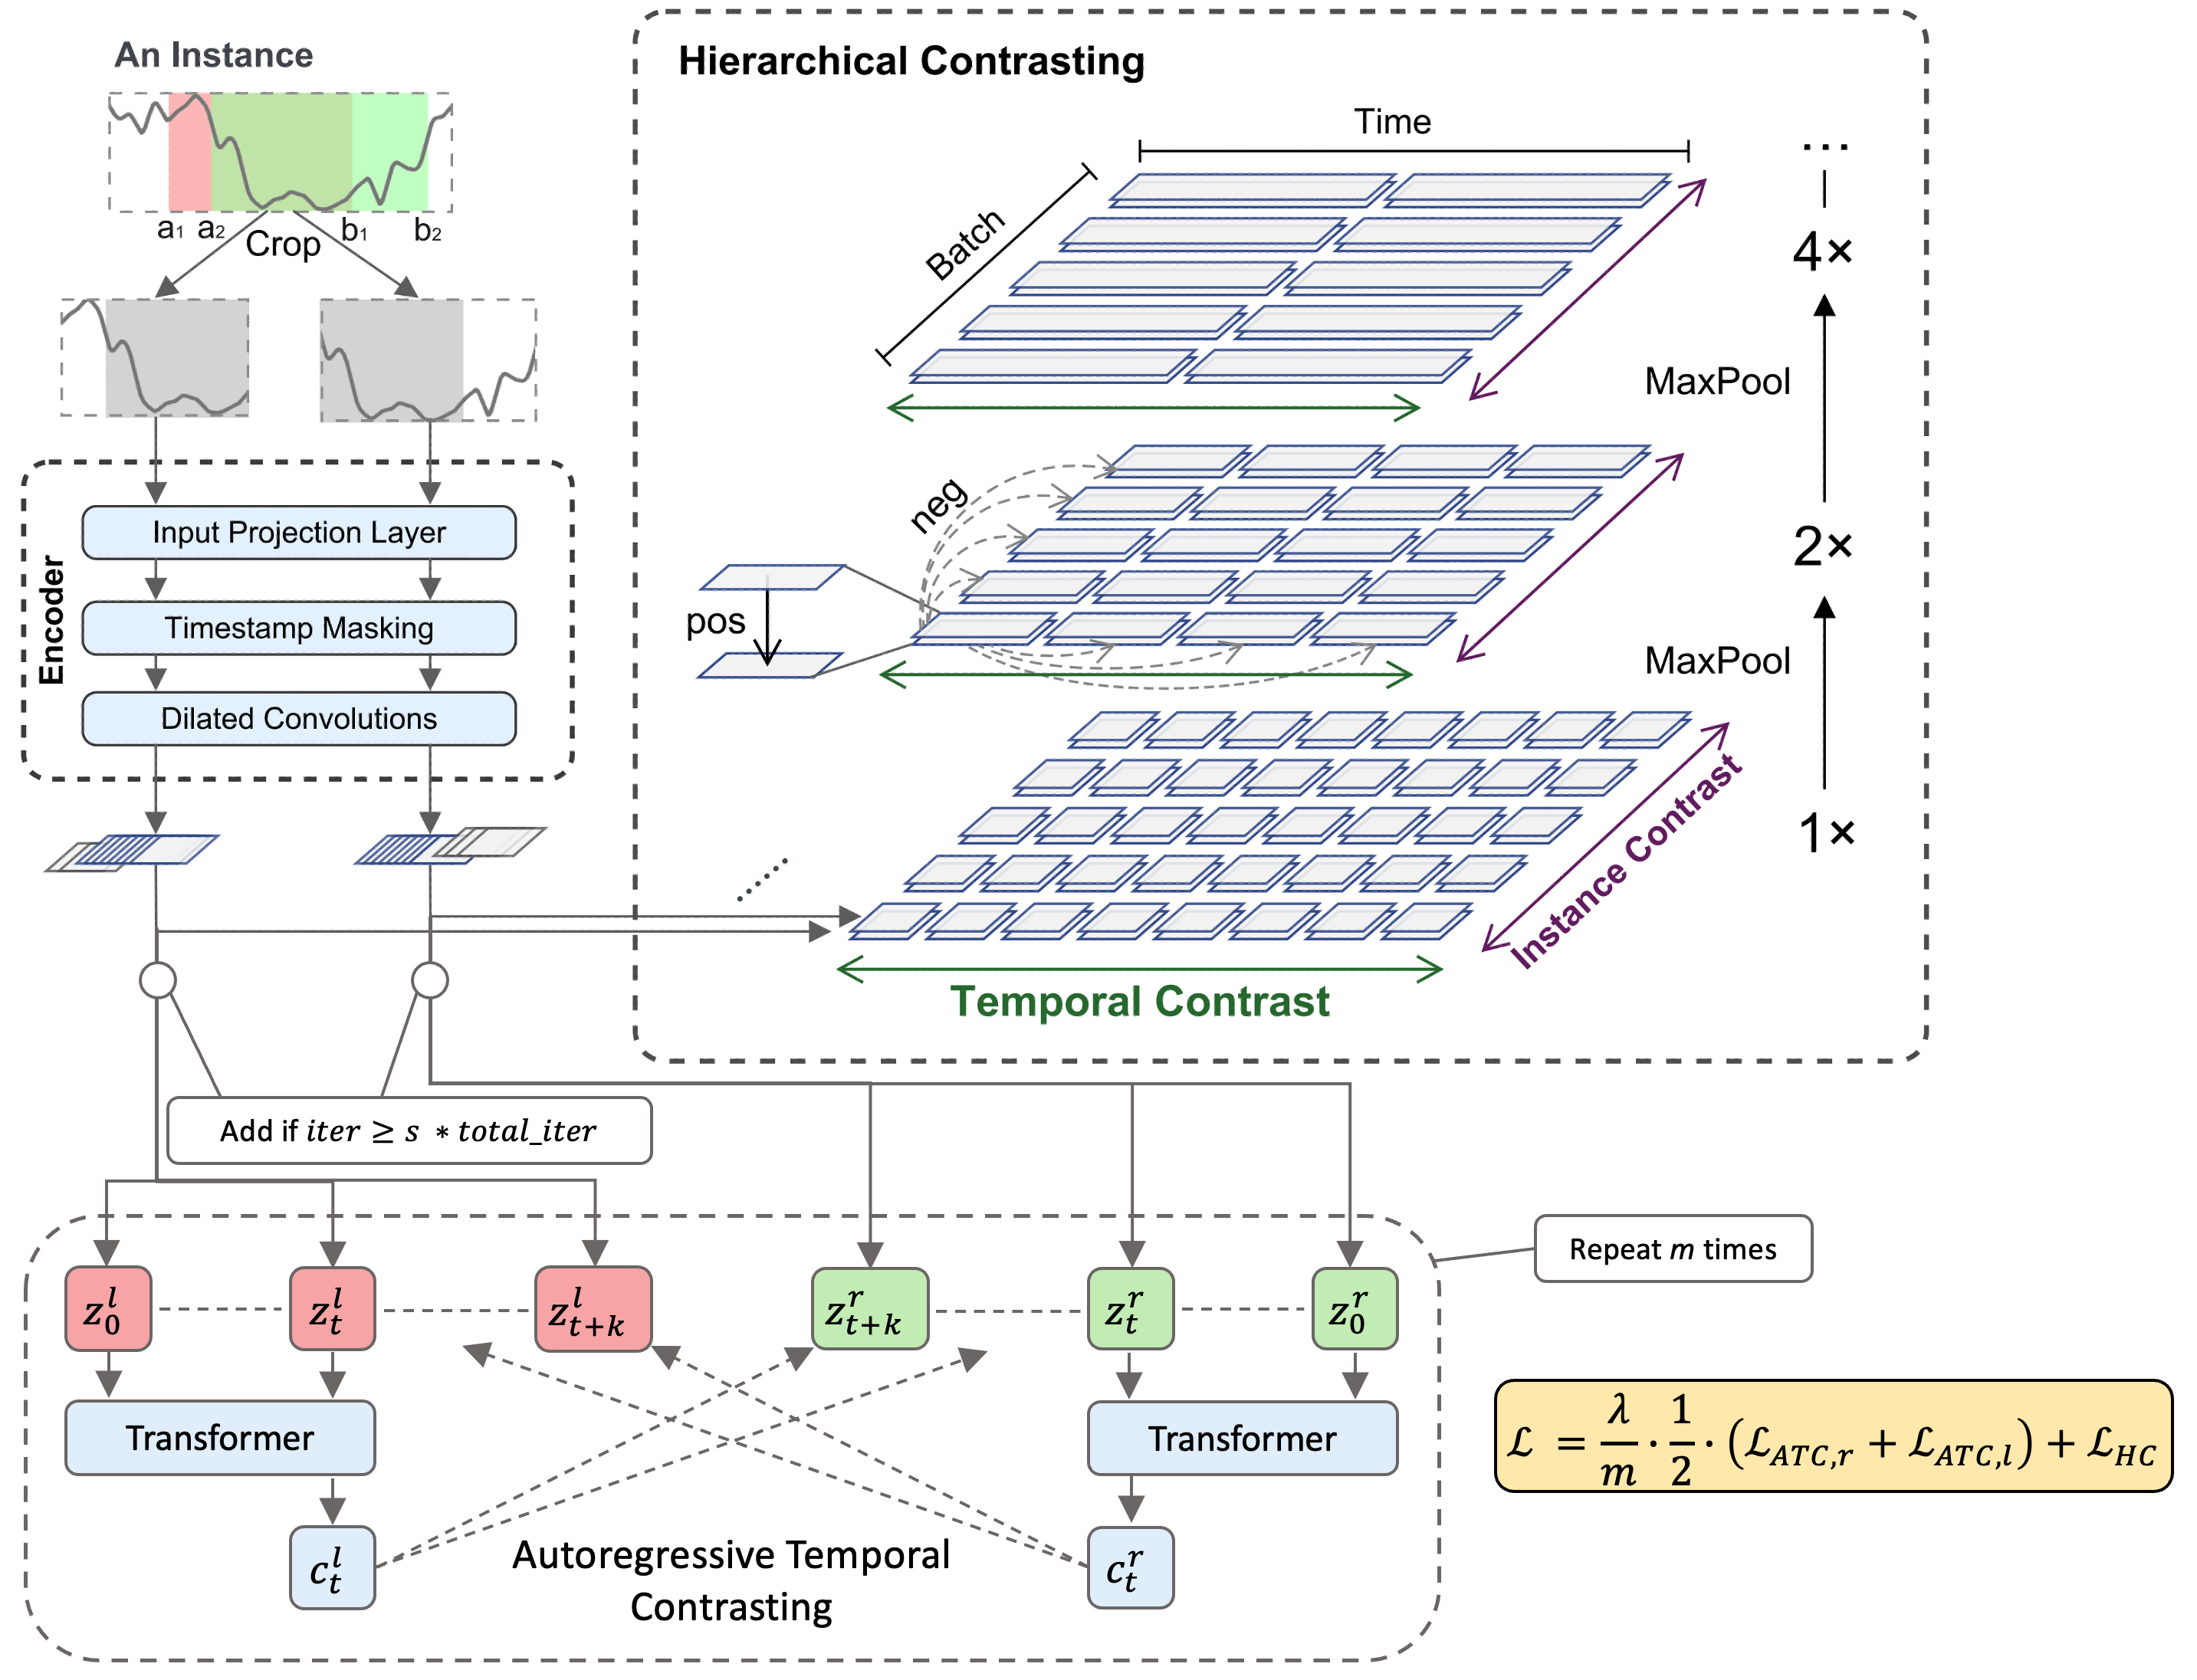
\includegraphics[width=1.0\textwidth]{fig/model_setup.png}
  \caption{Structure of model (TS2Vec part copied from \citet{ts2vec} and ATC part is own illustration based on \citet{tstcc})}
\end{figure}

In TS2Vec, two overlapping windows of a (multivariate) time series are sampled, where the left window is defined by $[a_{1}, b_{1}]$ and the right window by $[a_{2}, b_{2}]$. The following relationship has to hold for the cut-off points: $0 < a_{1} \leq a_{2} \leq b_{1} \leq b_{2} \leq T$. Each window is encoded separately by feeding it through an input projection layer, timestamp masking and dilated convolutions. The similarity of the overlapping part (i.e. $[a_{2}, b_{1}]$) of the encoded sequences in two different contexts is evaluated using hierarchical contrasting, applying temporal and instance contrasting iteratively. Temporal contrasting applies a contrastive loss over all time stamps of the same time series, where the same time stamps encoded in two representations are treated as positives and different time stamps as negatives. Instance contrasting, meanwhile, treats the two representations from different contexts of the same time series as positives and representations of different time series in the batch as negatives. By employing this two-fold loss function, the authors aim to achieve contextual consistency, which induces more robust learned representations. See \citet{ts2vec} for more details (\textcolor{red}{necessary?}). \\

As outlined above, temporal contrasting considers time stamps rather isolated. Thus, we integrated the idea by \citet{tstcc} to use an autoregressive model, which summarizes the latent representation into a context vector, into the TS2Vec framework. To be precise, all latent representations up to a randomly sampled timestamp $t$ (i.e. $\boldsymbol{z}_{<t}$) are passed to a Transformer, which summarizes them into a context vector $c_{t}$. This context vector is used to predict the next $k$ latent representations that were encoded from the other window (cross-prediction task). The prediction is evaluated using a contrastive loss over all time stamps in the prediction window. See \citet{tstcc} for more technical details. \\

The main adaptions are the following:
\begin{itemize}
\item While \citet{tstcc} use so-called strong and weak augmentations to induce latent representations of the time series in two different contexts, here two sampled and overlapping windows are used according to the TS2Vec model structure.
\item The autoregressive model may not be included until later iterations of the optimization, allowing the original TS2Vec component to induce reasonable latent representations that are refined by an autoregressive component at a later stage.
\item Since the context vector is only used to predict a limited number of $k$ consecutive latent representations at each iteration, the procedure of sampling $t$ and cross-predicting using a context vector can be repeated $m$ times to exploit a larger fraction of the time series.
\item The final loss function is the sum of the hierarchical contrastive loss and the mean of the two autoregressive temporal contrastive losses, which were derived by cross predicting the latent representations encoded from the left and right windows.
\item A relative importance parameter $\lambda$, rescaled by the number of repetitions of the cross-prediction task, is added.
\end{itemize}

\section{Experiments and results}

For comparability, we used the classification task of the whole time series as proposed by \citet{ts2vec} as a downstream task. \textcolor{red}{Why not other downstream tasks?}. This involved fitting an SVM classifier to the instance-level representation of the time series that had been derived by max-pooling over all individual timestamps. This allowed the classes of each instance to be predicted, and the performance was measured in terms of accuracy. \\

To perform experiments, we used the subset of 12 UEA datasets to benchmark against TS2Vec, on which \citet{ts2vec} reported SOTA performance in their paper. The convergence path of the adapted loss function for the StandWalkJump dataset as an example can be seen below. \\

\begin{figure}[H]
  \centering
  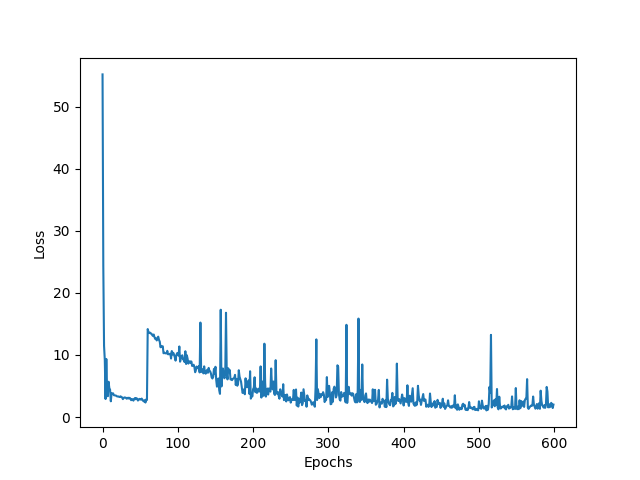
\includegraphics[width=0.7\textwidth]{fig/StandWalkJump_default_ar_2.png}
  \caption{Loss convergence of StandWalkJump dataset for s=0.1}
\end{figure}

The loss converges fairly quickly for the model without integrating the AR model. After 60 epochs, the loss jumps up since the additional objective of the AR model was added. The combined objective then converges to a similar low value as the initial model, although the convergence is not as smooth as without the combined objective. \\

Since our implementation was done in a slightly different Python environment, we compared TS2VecAR to the replicated results of TS2Vec with the default settings as specified in their repository. The results of the experiments\footnote{As hyperparemeters we chose $\lambda = 5$ since the ATC loss is smaller than the HC loss and $m=5$ to allow for sufficient cross prediction tasks in each iteration. All models were trained for the 600 iterations as specified default in TS2Vec.} are shown below, with different specifications of the share of iterations which did not include the autoregressive temporal contrasting component. \\

\begin{center}
\begin{tabular}{lrrrrl}
\toprule
                  Dataset &  AR (s=0) & AR (s=0.1) &  AR (s=0.2) &  Replicated &   Type \\
\midrule
       SelfRegulationSCP2 &              0.544 &                0.550 &                0.550 &       \textbf{0.556} &    EEG \\
            StandWalkJump &              \textbf{0.533} &                0.467 &                0.400 &       0.467 &    ECG \\
        SpokenArabicDigits &              0.967 &                0.959 &                0.977 &       \textbf{0.989} & Speech \\
            DuckDuckGeese &              0.460 &                0.460 &                \textbf{0.540} &       0.520 &  Audio \\
ArticularyWordRecognition &              \textbf{0.987} &                0.970 &                0.977 &       0.977 & Motion \\
    CharacterTrajectories &              0.991 &                0.993 &                \textbf{0.994} &       0.992 & Motion \\
               EigenWorms &              0.786 &                0.756 &                0.809 &       \textbf{0.863} & Motion \\
                 PenDigits &              0.988 &                0.986 &                \textbf{0.990} &       0.989 & Motion \\
              Handwriting &              \textbf{0.556} &               0.551 &                0.548 &       0.531 &    HAR \\
                   NATOPS &              0.911 &                0.839 &                0.878 &       \textbf{0.939} &    HAR \\
             RacketSports &              0.888 &                0.888 &                \textbf{0.895} &       0.855 &    HAR \\
      UWaveGestureLibrary &              0.919 &                \textbf{0.925} &                0.919 &       0.906 &    HAR \\
 \midrule
 Mean (All datasets) & 0.794 & 0.779 & 0.790 & \textbf{0.799} & \\
 Mean (HAR datasets) & \textbf{0.819} & 0.801 & 0.810 & 0.808 &  \\
\bottomrule
\end{tabular}
\end{center}

In 8 out of 12 datasets TS2Vec is outperformed by at least one specification of TS2VecAR. However, on average, TS2Vec still has the highest accuracy, partly due to the very low performance of the  $s=0$ and $s=1$ specifications in the DuckDuckGeese and Eigenworms datasets, and the $s=0.2$ specification in the StandWalkJump and EigenWorms and NATOPS datasets. \\

Considering only the subsample of Human Activity Recognition (HAR) datasets, TS2VecAR outperforms TS2Vec on three out of four datasets in all specifications.  On average, the improvement is $1.1\%$ when comparing the $s=0$ specification to TS2Vec. However, the for some datasets better individual performances can be achieved by including the autoregressive temporal contrasting after some initial training using only hierarchical contrasting. This suggests that it may be beneficial to first learn a better representation before using it for the cross-prediction task. However, the average accuracy for these specifications is compromised by the low performance on the NATOPS dataset.

\section{Conclusion}

TS2Vec has shown very strong results in learning robust latent representations of a time series via contextual contrasting, which can be used for various downstream task such as classification. However, the latent representation does not capture information about future time stamps, which would allow to learn more about the structure of the time series. Thus, TS2Vec can be extended by adding an autoregressive component in the learning process, which performs a cross-prediction task. This has shown better results for several datasets, where this study has in particular shown improvements for human activity recognition tasks.

\newpage

\bibliographystyle{apalike}
\bibliography{References}

%%%%%%%%%%%%%%%%%%%%%%%%%%%%%%%%%%%%%%%%%%%%%%%%%%%%%%%%%%%%

\end{document}